\documentclass[tikz,border=10pt]{standalone}
\usepackage{tikz}
\usetikzlibrary{shapes,arrows,positioning,calc,patterns,shadows,arrows.meta}

\definecolor{bertblue}{RGB}{66,133,244}
\definecolor{gptgreen}{RGB}{52,168,83}
\definecolor{padgray}{RGB}{200,200,200}
\definecolor{realtoken}{RGB}{255,255,255}
\definecolor{sepviolet}{RGB}{142,36,245}
\definecolor{clsorange}{RGB}{251,188,5}

\begin{document}
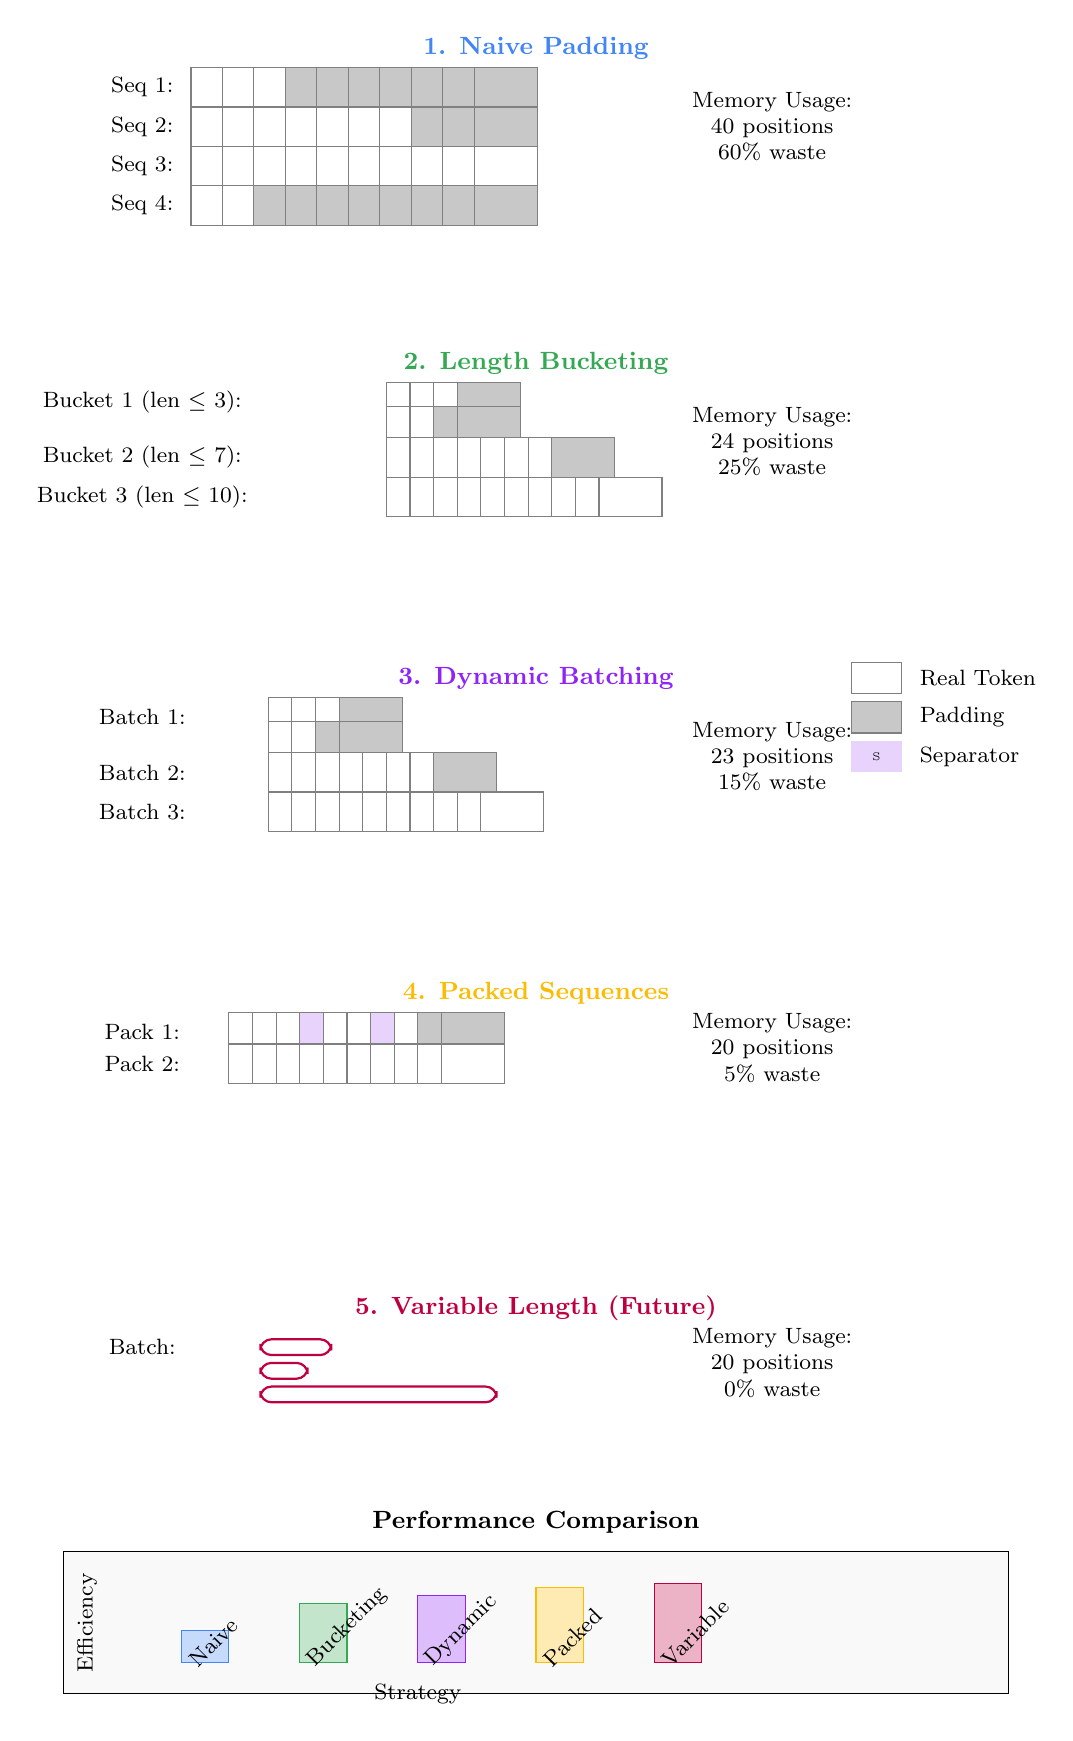
\begin{tikzpicture}[
    token/.style={rectangle, minimum width=0.8cm, minimum height=0.5cm, font=\tiny},
    realtoken/.style={token, fill=realtoken, draw=black!50},
    padtoken/.style={token, fill=padgray, draw=black!50},
    label/.style={font=\footnotesize},
    title/.style={font=\small\bfseries}
]

% === VERTICAL ARRANGEMENT DOCUMENTATION ===
% Each strategy positioned vertically with y spacing of 5cm
% Strategy 1: y=18, Strategy 2: y=14, Strategy 3: y=10, Strategy 4: y=6, Strategy 5: y=2
% Performance chart at bottom: y=-2
% Legend positioned on right side

% Strategy 1: Naive Padding
\node[title, bertblue] at (6, 18) {1. Naive Padding};

% Sequences with different lengths - using consistent positioning
\node[label] (seq1-label) at (1, 17.5) {Seq 1:};
\foreach \i in {0,...,2} {
    \node[realtoken] at ($(seq1-label.east)+(0.5+\i*0.4,0)$) {};
}
\foreach \i in {3,...,9} {
    \node[padtoken] at ($(seq1-label.east)+(0.5+\i*0.4,0)$) {};
}

\node[label] (seq2-label) at (1, 17) {Seq 2:};
\foreach \i in {0,...,6} {
    \node[realtoken] at ($(seq2-label.east)+(0.5+\i*0.4,0)$) {};
}
\foreach \i in {7,...,9} {
    \node[padtoken] at ($(seq2-label.east)+(0.5+\i*0.4,0)$) {};
}

\node[label] (seq3-label) at (1, 16.5) {Seq 3:};
\foreach \i in {0,...,9} {
    \node[realtoken] at ($(seq3-label.east)+(0.5+\i*0.4,0)$) {};
}

\node[label] (seq4-label) at (1, 16) {Seq 4:};
\foreach \i in {0,...,1} {
    \node[realtoken] at ($(seq4-label.east)+(0.5+\i*0.4,0)$) {};
}
\foreach \i in {2,...,9} {
    \node[padtoken] at ($(seq4-label.east)+(0.5+\i*0.4,0)$) {};
}

% Memory usage calculation
\node[label, align=center] at (9, 17) {Memory Usage:\\40 positions\\60\% waste};

% Strategy 2: Length Bucketing
\node[title, gptgreen] at (6, 14) {2. Length Bucketing};

% Bucket 1: Short sequences
\node[label] at (1, 13.5) {Bucket 1 (len $\leq$ 3):};
\foreach \i in {0,...,2} {
    \node[realtoken] at (4.5+\i*0.3, 13.5) {};
}
\node[padtoken] at (4.5+3*0.3, 13.5) {};

\foreach \i in {0,...,1} {
    \node[realtoken] at (4.5+\i*0.3, 13.2) {};
}
\foreach \i in {2,3} {
    \node[padtoken] at (4.5+\i*0.3, 13.2) {};
}

% Bucket 2: Medium sequences
\node[label] at (1, 12.8) {Bucket 2 (len $\leq$ 7):};
\foreach \i in {0,...,6} {
    \node[realtoken] at (4.5+\i*0.3, 12.8) {};
}
\node[padtoken] at (4.5+7*0.3, 12.8) {};

% Bucket 3: Long sequences
\node[label] at (1, 12.3) {Bucket 3 (len $\leq$ 10):};
\foreach \i in {0,...,9} {
    \node[realtoken] at (4.5+\i*0.3, 12.3) {};
}

\node[label, align=center] at (9, 13) {Memory Usage:\\24 positions\\25\% waste};

% Strategy 3: Dynamic Batching
\node[title, sepviolet] at (6, 10) {3. Dynamic Batching};

% Batch 1: Similar lengths
\node[label] at (1, 9.5) {Batch 1:};
\foreach \i in {0,...,2} {
    \node[realtoken] at (3+\i*0.3, 9.5) {};
}
\node[padtoken] at (3+3*0.3, 9.5) {};

\foreach \i in {0,...,1} {
    \node[realtoken] at (3+\i*0.3, 9.2) {};
}
\foreach \i in {2,3} {
    \node[padtoken] at (3+\i*0.3, 9.2) {};
}

% Batch 2: Similar lengths
\node[label] at (1, 8.8) {Batch 2:};
\foreach \i in {0,...,6} {
    \node[realtoken] at (3+\i*0.3, 8.8) {};
}
\node[padtoken] at (3+7*0.3, 8.8) {};

% Batch 3: Long sequence alone
\node[label] at (1, 8.3) {Batch 3:};
\foreach \i in {0,...,9} {
    \node[realtoken] at (3+\i*0.3, 8.3) {};
}

\node[label, align=center] at (9, 9) {Memory Usage:\\23 positions\\15\% waste};

% Strategy 4: Packed Sequences
\node[title, clsorange] at (6, 6) {4. Packed Sequences};

% Pack multiple short sequences together
\node[label] at (1, 5.5) {Pack 1:};
\foreach \i in {0,...,2} {
    \node[realtoken] at (2.5+\i*0.3, 5.5) {};
}
\node[realtoken, fill=sepviolet!20] at (2.5+3*0.3, 5.5) {S}; % Separator
\foreach \i in {4,...,5} {
    \node[realtoken] at (2.5+\i*0.3, 5.5) {};
}
\node[realtoken, fill=sepviolet!20] at (2.5+6*0.3, 5.5) {S}; % Separator
\foreach \i in {7,...,7} {
    \node[realtoken] at (2.5+\i*0.3, 5.5) {};
}
\foreach \i in {8,...,9} {
    \node[padtoken] at (2.5+\i*0.3, 5.5) {};
}

\node[label] at (1, 5.1) {Pack 2:};
\foreach \i in {0,...,9} {
    \node[realtoken] at (2.5+\i*0.3, 5.1) {};
}

\node[label, align=center] at (9, 5.3) {Memory Usage:\\20 positions\\5\% waste};

% Strategy 5: Variable Length (Future)
\node[title, color=purple] at (6, 2) {5. Variable Length (Future)};

% Irregular shapes representing variable-length processing
\node[label] at (1, 1.5) {Batch:};
\draw[thick, purple, rounded corners] (2.5, 1.6) -- (3.4, 1.6) -- (3.4, 1.4) -- (2.5, 1.4) -- cycle;
\draw[thick, purple, rounded corners] (2.5, 1.3) -- (3.1, 1.3) -- (3.1, 1.1) -- (2.5, 1.1) -- cycle;
\draw[thick, purple, rounded corners] (2.5, 1.0) -- (5.5, 1.0) -- (5.5, 0.8) -- (2.5, 0.8) -- cycle;

\node[label, align=center] at (9, 1.3) {Memory Usage:\\20 positions\\0\% waste};

% Performance comparison chart - at bottom
\node[rectangle, draw=black, fill=gray!5, minimum width=12cm, minimum height=1.8cm] (chart) at (6, -2) {};
\node[title, above=0.1cm of chart.north] {Performance Comparison};

% Bar chart showing efficiency
\foreach \strategy/\x/\color/\height in {Naive/1.5/bertblue/0.4, Bucketing/3/gptgreen/0.75, Dynamic/4.5/sepviolet/0.85, Packed/6/clsorange/0.95, Variable/7.5/purple/1.0} {
    \draw[fill=\color!30, draw=\color] (\x, -2.5) rectangle ++(0.6, \height);
    \node[label, rotate=45, anchor=west] at (\x+0.05, -2.6) {\strategy};
}

\node[label, rotate=90] at (0.3, -2) {Efficiency};
\node[label] at (4.5, -2.9) {Strategy};

% Legend - positioned on right side
\begin{scope}[every node/.style={label, anchor=west}]
    \node[realtoken, scale=0.8] (real-legend) at (10, 10) {};
    \node at ($(real-legend.east)+(0.1,0)$) {Real Token};
    \node[padtoken, scale=0.8] (pad-legend) at (10, 9.5) {};
    \node at ($(pad-legend.east)+(0.1,0)$) {Padding};
    \node[token, fill=sepviolet!20, scale=0.8] (sep-legend) at (10, 9) {S};
    \node at ($(sep-legend.east)+(0.1,0)$) {Separator};
\end{scope}

\end{tikzpicture}
\end{document}